\section{Historical pseudoexperiment regimes and model decisions}
\label{app:v501-historical-methods}
This appendix restores the three generation regimes and full-100 exposure
study from the v4.9.7 note, together with the threshold and length-scale
studies that explain subsequent decisions. Their original data fractions,
statistical conventions and GP policies remain identified. They are
historical validation evidence, not additional versions of the current
observed curves.

\subsection{Three toy-generation regimes}
\label{sec:v501-toy-regimes}
The word ``toy'' does not specify what is allowed to fluctuate. The three
regimes below test different parts of the analysis and cannot be pooled
into one calibration sample.

\paragraph{Analytic functional-form pseudoexperiments.}
A smooth function is fitted to a source spectrum independently of the GP.
Its integral in each native bin supplies a background mean, and independent
Poisson counts generate the full spectrum. The GP is then retrained on
that spectrum's sidebands before extraction. This tests recovery under a
declared alternative shape, including the response of the training step.
The exact year-matched and generalized-gamma families are written in
Eqs.~\ref{eq:v501-shifted-seed}--\ref{eq:v501-gengamma-seed}. Parameters
are chosen using source-fit and normalization checks before extraction;
a selected function is not refitted to obtain a more favorable signal pull.

\paragraph{Conditional blind-window GP toys.}
The observed sidebands are fitted once at a specified mass, giving a
background mean and correlated uncertainty inside the excluded window.
A background realization and a signal are sampled using that fixed
prediction, and only the local extraction is repeated. This isolates the
response of the likelihood under its assumed background uncertainty.
It omits the variation in sideband fitting, hyperparameter estimation and
model selection. It is therefore a conditional extraction test or an
expected-limit reference under the stated posterior model, rather than
an independent test of GP interpolation.

\paragraph{Full-spectrum GP-mean/refit pseudoexperiments.}
The propagated count-space GP mean provides an expected background over
the complete support. A full spectrum is sampled, the complete Gaussian
signal is added, and the sideband-to-window prediction is re-estimated
before extraction. Signal tails outside the mask participate in the
new training sample, allowing the study to diagnose signal absorption.
The generation remains conditional on a GP-derived truth. Whether kernel
coordinates are reoptimized or frozen is a separate analysis choice:
the historical full-refit studies reoptimize them, while the later
calibration and significance-GP studies condition on the reviewed kernels.

\begin{table}[H]\centering\small
\begin{tabularx}{\linewidth}{P{0.24\linewidth}P{0.29\linewidth}Y}
\toprule
Regime & Background source and repeated steps & Principal question\\\midrule
Analytic full spectrum & Independent smooth source fit; Poisson bins;
new GP sideband fit & Can the analysis recover signals from this
alternative smooth spectrum?\\
Conditional GP window & Fixed sideband prediction and covariance;
repeat local likelihood & Does extraction propagate the uncertainty
represented by this fixed local model?\\
GP-mean full spectrum & GP-derived full-support mean; new spectrum
and sideband prediction & How does retraining respond to fluctuations
and signal tails under this GP-conditioned truth?\\\bottomrule
\end{tabularx}
\caption{Restored classification of the three historical generation
regimes. The term ``full spectrum'' alone does not imply that kernel
optimization or all preceding model choices were repeated.}
\label{tab:v501-toy-regimes}
\end{table}

Signal sampling is another independent choice. Poisson-total injection
samples each bin with mean $A_{\rm inj}w_i$; a fixed-total multinomial
injection fluctuates only the allocation among bins. Fixed-total
background scans are likewise conditional on their chosen event total.
The full-100 study below used Poisson signal injection, while its mean
strength was set by each background toy's matched reference fit. Thus
neither its reference error nor its physical injected yield is constant
across the ensemble. These details distinguish it from the later
fixed-physical-yield calibration.

\subsection{Historical full-100 2021 source-and-exposure closure}
\label{sec:v501-v4p6-exposure-refmatched-full100}

\paragraph{Finding summary.}
The archived complete ensemble confirmed a local conditional 65~MeV offset in the
$1\%\times10$ lane, with a smaller native-10\% response, after a pull-blind
optimizer treatment.  It does not establish observed-data bias or direct coverage.

This restored v4.9.7 Appendix B.6 records the complete 100-background
ensembles before the later threshold replacements. Its 95\% intervals and
original generating truths remain distinct from the 90\% intervals of the
updated main-text composite.  It was frozen before the reserve toys were inspected:
toys 0--9 are the pilot sample and toys 10--99 are an independent confirmation
sample for the pilot-selected $1\%\times10$, 65~MeV zero-signal offset.  All 100
background pseudo-histograms are refitted uniformly under the new estimator and
restart policy; the v4.5 extraction rows are not pooled with the new rows.

The analysis card remains the declared v4.2 2021 state: a 40--300~MeV GP support,
50--250~MeV search range, $k_{\min}=1.1$, $k_{\max}=15$, a
$2.25\sigma_m$ blind and training exclusion, two required sidebands, five-bin local
rebinning, and 12 randomized optimizer restarts in addition to the nominal start.
The four historical ensembles are $1\%\times10$, native 10\%, $1\%\times100$, and
$10\%\times10$.  The common \texttt{fGenGammaThresh} family is fitted independently
to the native 1\% and native 10\% spectra.  These functions are smooth stress truths,
not physical background generators.  In particular, the native-10\% fit has Pearson
$\chi^2/\mathrm{ndf}=2.781$ and is deliberately not retuned after inspecting closure.

For each scenario $s$, background toy $t$, and mass $m$, an independently optimized
matched background-only fit defines $\sigma^{\mathrm{ref}}_{A,stm}$.  The injected
amplitude and reported pull are
\begin{equation}
 A^{\mathrm{inj}}_{stmz}=z\,\sigma^{\mathrm{ref}}_{A,stm},
 \qquad
 p_{stmz}=\frac{\widehat A_{stmz}-A^{\mathrm{inj}}_{stmz}}
 {\widehat\sigma_{A,stmz}},
 \qquad z\in\{0,1,3,5\}.
 \label{eq:v501-v4p6-refmatched-pull}
\end{equation}
The injection scale is therefore toy-local, while the denominator is always the
post-fit uncertainty of the injected pseudoexperiment.  The exact v4.2 conversion
$K_{stm}=A(\eps^2=1)$ is also recomputed from each native pseudo-spectrum, including
the $\pm1.64\sigma_m$ fractional-bin density integral, so that
\begin{equation}
 \eps^2_{\mathrm{inj},stmz}=A^{\mathrm{inj}}_{stmz}/K_{stm},
 \qquad
 \widehat{\eps^2}_{stmz}=\widehat A_{stmz}/K_{stm}.
 \label{eq:v501-v4p6-eps2-coordinate}
\end{equation}
Negative fitted coordinates are retained.  They are estimator fluctuations, not
physical negative couplings, and none of these distributions is an upper limit or an
expected-limit band.

\begin{figure}[p]
\centering
\graphicorplaceholder{0.99\linewidth}{../figures/history_writer/full100_functional_form_exposure_mass_distributions_full100.pdf}
\caption{Invariant-mass construction of the full-100 ensembles, following the
functional-form display of Fig.~\ref{fig:v491-functional-form-seed-overview}.  Each row
shows the native source and independently fitted stress truth (left), the scaled
analytic expectation with the mean, median, and central 68\% range of 100 background
pseudoexperiments (middle), and the toy-mean residual divided by its expected standard
error (right).  Grey bands are support-only regions outside the 50--250~MeV search.
The common analytic family isolates source/selection and normalization differences
without claiming that either smooth function is a physical background generator.}
\label{fig:v501-v4p6-functional-form-exposure-distributions}
\end{figure}

\subsubsection{Predeclared optimizer-repeat and exclusion gate}

Each optimizer attempt refits exactly the same cached background and signal counts;
the pseudoexperiment seed and optimizer-start seed occupy separate deterministic
namespaces.  An attempt uses the nominal kernel start plus 12 randomized starts and
archives its seed, warnings, log marginal likelihood (LML), length scale, constant,
extraction uncertainty, and covariance diagnostics.  Three independently seeded,
identically configured background-only/zero-signal optimizer attempts use the same
data and masks.  The highest-LML branch
must occur at least twice under the predeclared agreement criteria
\begin{equation}
 \frac{|\Delta\mathrm{LML}|}{N_{\mathrm{train}}}\leq10^{-3},\quad
 |\Delta\ln\ell|\leq0.01,\quad
 |\Delta\ln C|\leq0.05,\quad
 |\Delta\ln\sigma_A|\leq0.02.
 \label{eq:v501-v4p6-branch-replication}
\end{equation}
If it does not, two additional independent attempts are made.  A nonzero-injection
fit begins with one attempt and receives two, then at most five, attempts if it has an
invalid or nonfinite fit/covariance state, retains the exact optimizer-start signature, lies
within 2\% of a length-scale bound, or has
$\widehat\sigma_A/\sigma_A^{\mathrm{ref}}\notin[0.5,2]$.  Branch selection uses only
maximum GP LML and reproducibility---never $\widehat A$, pull sign or size,
$\widehat\eps^2$, or agreement with the injected amplitude.
Optimizer warnings are archived for audit, but are not by themselves a repeat or
exclusion trigger; only the pull- and amplitude-blind numerical diagnostics listed above
activate the adaptive attempts.

An irreproducible reference state excludes all four strengths at that
scenario--toy--mass key; an irreproducible injected refit excludes only that strength.
Statistical extremes that pass this pull-blind technical gate remain accepted;
repeat-triggered boundary solutions are retained when replicated.  A closure cell
was predeclared reportable only if at least 95 of its 100 generated rows survived.
This fit-state policy avoids both post-hoc pull clipping and the scientifically
incorrect removal of a complete pseudoexperiment because it fluctuates unfavorably.

The production run contains 400 scenario--toy tasks, 8000 predeclared extraction-state
keys, 7996 finite raw amplitude fits, and 12,845 archived optimizer-attempt records.
Of the 7994 accepted states,
5593 required one attempt, 2384 required three, and 17 required five.  Six states are
excluded: the $1\%\times100$ toy-83, 90~MeV, $z=3$ refit; the $10\%\times10$
toy-28, 180~MeV, $z=5$ refit; and all four strengths of the $10\%\times10$ toy-66,
90~MeV reference state.  The first two fail injected-fit reproducibility and the last
fails reference-branch reproducibility after five attempts.  No entire background-toy
index is removed, every one of the 80 closure cells retains 99 or 100 rows, and all pass the
predeclared minimum-size gate.

The count-space covariance produced by the frozen lognormal-moment mapping is
classified as numerically repairable, not necessarily positive semidefinite, when it
is finite and symmetric and satisfies
$\lambda_{\min}/\max_i|C_{ii}|\geq-0.01$.  The extraction likelihood then follows its
frozen numerical path: progressively larger diagonal jitter through
$10^{-3}\max_i|C_{ii}|$, followed, when needed, by an eigenvalue-clipped square root.
Among the 7994 accepted states, 498 archived raw matrices have the eigenvalue ratio
below $-10^{-3}$ and 22 lie below $-0.005$; the latter are confined to 90~MeV in the
two high-exposure ensembles.  A pull-blind influence check that omits those 22 rows
changes any closure-cell mean by at most 0.031 and any width by at most 0.014, but
would reduce one cell below the predeclared 95-row reporting threshold.  The rows
therefore remain in the headline moments.  An all-state deterministic reconstruction
replays the actual repair path and compares it with the minimally sufficient isotropic
diagonal loading.  The replay agrees with the archived pull to within 0.0031 and with
its uncertainty to within $3.2\times10^{-4}$ relatively; changing to minimal diagonal
loading moves any pull by at most 0.0029 and any uncertainty by at most
$6.94\times10^{-4}$ relatively; the largest changes in a cell mean and width are
$5.0\times10^{-5}$ and $1.1\times10^{-4}$, respectively.  The archived ratios, rather than reconstructed
threshold counts, define the 498 and 22 figures above.  This tolerance and repair audit is a
numerical qualification of the estimator, not evidence that the unrepaired matrices
are positive semidefinite.

\begin{figure}[p]
\centering
\graphicorplaceholder{0.99\linewidth}{../figures/history_writer/full100_optimizer_gate_diagnostics_full100.pdf}
\caption{Optimizer-repeat gate and exclusion audit.  The upper-left panel compares
zero-signal means from the raw first attempts with the accepted LML-selected states;
the visibly repaired $1\%\times100$, 65~MeV point is numerical rather than a pull-based
deletion.  The upper-right panel reports accepted factor-15 contacts.  The lower-left
panel gives the adaptive attempt workload, and the lower-right panel lists all six
excluded states.  Statistical extremes that pass the pull-blind technical gate remain
in the headline summaries; repeat-triggered boundary solutions are retained when
replicated.}
\label{fig:v501-v4p6-optimizer-gate}
\end{figure}

\subsubsection{Spurious-signal bias and independent confirmation}

Figure~\ref{fig:v501-v4p6-zero-signal-spurious} isolates the $z=0$ tests.  The apparent
$1\%\times10$, 65~MeV pilot offset does not disappear with more toys.  In the
predeclared independent reserve (toys 10--99), the mean pull is
$0.768$ with sample width $0.944$ and 95\% Student-$t$ interval
$[0.570,0.965]$; the two-sided test of zero mean gives
$p=1.64\times10^{-11}$.  This exceeds the predeclared materiality threshold
$|\bar p|\geq0.2$.  The full-100 precision estimate is
$0.789$ with width $0.962$, median $0.784$, and 95\% interval
$[0.598,0.980]$.

The deterministic analytic-mean stress spectrum gives a stable zero-signal pull of
$0.837$ at the same mass.  The agreement with the 100-toy mean and the near-normal
reserve quantiles in Fig.~\ref{fig:v501-v4p6-bias-confirmation} identify a local
functional-form/GP underprediction, not an optimizer failure or a few statistical
outliers.  The four injection strengths share each background toy and are highly
correlated; their similar offsets are recovery diagnostics, not four independent
confirmations.

The remaining zero-signal cells were treated as exploratory with Holm correction over
all 20 scenario--mass checks.  Two additional material offsets survive that correction:
native 10\% at 65~MeV has mean $0.716$ (analytic-mean value $0.723$), and
$10\%\times10$ at 180~MeV has mean $0.338$ (analytic-mean value $0.194$).
These are closure properties conditional on the deliberately imperfect smooth stress
truth and the frozen card.  They do not measure a bias of the observed data result and
do not calibrate frequentist coverage.

\begin{figure}[p]
\centering
\graphicorplaceholder{0.99\linewidth}{../figures/history_writer/full100_spurious_signal_zero_sigma_full100.pdf}
\caption{Full-100 spurious-signal study.  Each row corresponds to one ensemble.  The
left panels show every accepted zero-signal pull and its median; the middle panels show
raw first-attempt means, accepted means with 95\% Student-$t$ intervals, and the
deterministic analytic-mean closure; the right panels show accepted sample widths with
95\% normal-theory intervals.  Red crosses mark excluded raw fit states where present.
No accepted pull is clipped.  The common mass dependence between analytic-mean and
ensemble results diagnoses stress-truth/model closure rather than a statistical
outlier.}
\label{fig:v501-v4p6-zero-signal-spurious}
\end{figure}

\begin{figure}[p]
\centering
\graphicorplaceholder{0.96\linewidth}{../figures/history_writer/full100_onepct_x10_65mev_bias_confirmation.pdf}
\caption{Investigation of the $1\%\times10$, 65~MeV closure offset.  The top-left
panel separates the pilot and independent reserve distributions; the top-right tracks
the running mean and its 95\% Student-$t$ interval, with the pilot/reserve boundary
fixed at toy 10.  The lower-left normal Q--Q diagnostic shows no isolated tail capable
of explaining the mean, and the lower-right panel shows the correlated response across
injection strengths.  The analytic-mean pull of 0.837 was obtained from the exact
stress-truth mean with independent optimizer seeds.}
\label{fig:v501-v4p6-bias-confirmation}
\end{figure}

\subsubsection{Injection recovery, pull widths, and signed coupling coordinates}

Figures~\ref{fig:v501-v4p6-closure-1pct-x10}--\ref{fig:v501-v4p6-closure-10pct-x10}
use a four-panel layout for mean pull, pull width, residual fitted
significance and recovered amplitude.  The pull-mean error bars are 95\% Student-$t$
intervals and the width bars are exact normal-theory intervals based on the accepted
sample size.  The lower panels show residual fitted significance and median amplitude
recovery with empirical central 68\% spreads.  Joining lines connect only the five
predeclared mass points.

\begin{figure}[p]
\centering
\graphicorplaceholder{0.97\linewidth}{../figures/history_writer/full100_refmatched_closure_full100_2021_1pct_x10.pdf}
\caption{Full-100 refmatched closure for $1\%\times10$.  Every cell retains 100
accepted toys.  The persistent positive 65~MeV pull means and the corresponding
analytic-mean result are local stress-truth/model offsets; the other masses have
near-unit widths and substantially smaller means.  Crosses in the mean panel show raw
first-attempt moments before the predeclared LML/reproducibility selection.}
\label{fig:v501-v4p6-closure-1pct-x10}
\end{figure}

\begin{figure}[p]
\centering
\graphicorplaceholder{0.97\linewidth}{../figures/history_writer/full100_refmatched_closure_full100_2021_10pct.pdf}
\caption{As in Fig.~\ref{fig:v501-v4p6-closure-1pct-x10}, for the native-10\% ensemble.
All cells retain 100 toys.  The largest mean offset is at 65~MeV.  The only accepted
width outside 0.8--1.2 in the complete study is 1.237 for the 65~MeV, $z=5$ cell; its
normal-theory 95\% interval is $[1.086,1.437]$.}
\label{fig:v501-v4p6-closure-10pct}
\end{figure}

\begin{figure}[p]
\centering
\graphicorplaceholder{0.97\linewidth}{../figures/history_writer/full100_refmatched_closure_full100_2021_1pct_x100.pdf}
\caption{As in Fig.~\ref{fig:v501-v4p6-closure-1pct-x10}, for $1\%\times100$.  The
90~MeV, $z=3$ cell retains 99 toys after one irreproducible injected refit is excluded;
all other cells retain 100.  Eighty-five of 1999 accepted fits contact the factor-15
upper length-scale bound.  Stable contacts are reported rather than removed or used to
change the frozen card.}
\label{fig:v501-v4p6-closure-1pct-x100}
\end{figure}

\begin{figure}[p]
\centering
\graphicorplaceholder{0.97\linewidth}{../figures/history_writer/full100_refmatched_closure_full100_2021_10pct_x10.pdf}
\caption{As in Fig.~\ref{fig:v501-v4p6-closure-1pct-x10}, for $10\%\times10$.  The four
90~MeV cells and the 180~MeV, $z=5$ cell retain 99 toys; all others retain 100.  The
repeat gate repairs the dramatic 65 and 180~MeV optimizer branches seen in the v4.5
pilot without discarding those background pseudoexperiments.  Among 1995 accepted
fits, 134 stably contact the factor-15 upper bound.}
\label{fig:v501-v4p6-closure-10pct-x10}
\end{figure}

\clearpage
\begin{table}[H]
\centering
\small
\caption{Full-100 accepted closure summary over the five requested masses.  The
maximum mean entries give the mass, and for nonzero injections also $z$, at which the
maximum absolute mean occurs.  Width ranges span five zero-signal or 15 nonzero cells.
Boundary contacts are accepted, stable fit states, not exclusions.}
\label{tab:v501-v4p6-refmatched-summary}
\begin{tabular}{lccccc}
\toprule
Ensemble & minimum $n$ & max $|\bar p|$, $z=0$ & width range, $z=0$ &
max $|\bar p|$, $z>0$ & width range, $z>0$ \\
\midrule
$1\%\times10$  & 100 & 0.789 (65)  & 0.962--1.138 & 0.760 (65, 1)  & 0.964--1.142 \\
native 10\%     & 100 & 0.716 (65)  & 0.923--1.142 & 0.689 (65, 1)  & 0.921--1.237 \\
$1\%\times100$ &  99 & 0.280 (120) & 0.884--1.088 & 0.378 (120, 5) & 0.879--1.131 \\
$10\%\times10$ &  99 & 0.338 (180) & 0.893--1.060 & 0.359 (120, 5) & 0.890--1.177 \\
\bottomrule
\end{tabular}
\end{table}

The accepted upper-bound occupancies are 0/2000 for $1\%\times10$, 0/2000 for
native 10\%, 85/1999 (4.25\%) for $1\%\times100$, and 134/1995 (6.72\%) for
$10\%\times10$.  The last two totals correspond to 23 and 37 unique
scenario--toy--mass states (14 and 18 unique toy indices), respectively, because
strengths sharing one background toy are correlated.  Factor 15 is therefore still a frozen candidate-card choice with
non-negligible high-exposure boundary contact, not a universally nonbinding bound.
Changing this upper bound would require a separate study using the same
datasets, followed by checks of the observed fits and coverage.

\begin{figure}[p]
\centering
\graphicorplaceholder{0.99\linewidth}{../figures/history_writer/full100_eps2_coordinate_distributions_full100.pdf}
\caption{Signed $\eps^2$ extraction-coordinate distributions for the 1-, 3-, and
5-$\sigma_A$ injections.  Points are all accepted fits; solid summaries are medians
and empirical 16--84\% intervals, while dashed summaries describe the toy-local
injected coordinates.  Panel-wise symmetric-log axes retain negative fitted values
and broad 1-$\sigma$ fluctuations.  Because both $K_{stm}$ and
$\sigma^{\mathrm{ref}}_{A,stm}$ are toy-local, the injected coordinates are
distributions.  These are extraction diagnostics, not limits, physical negative
couplings, or expected bands.}
\label{fig:v501-v4p6-eps2-distributions}
\end{figure}

\begin{figure}[p]
\centering
\graphicorplaceholder{0.99\linewidth}{../figures/history_writer/full100_direct_pairwise_eps2_comparisons_full100.pdf}
\caption{Direct full-100 comparisons between native 10\% and $1\%\times10$ (top)
and between $10\%\times10$ and $1\%\times100$ (bottom).  Solid curves and bands are
fitted medians and empirical 16--84\% spreads; dashed curves are injected medians.
The source functions are fitted independently and the cross-source ensembles are
unpaired.  Their expected-normalization ratio is 1.1296466 in both comparisons, so
differences combine source/selection shape and normalization and are not pure exposure
effects or paired tests.  The ribbons are descriptive coordinate spreads, not
expected-limit bands.}
\label{fig:v501-v4p6-direct-eps2-comparisons}
\end{figure}

\clearpage
The full ensemble resolves the principal v4.5 ambiguity.  The two spectacular pilot
branches were numerical and are repaired by reproducible maximum-LML selection, while
the $1\%\times10$, 65~MeV offset is a stable local closure failure of the declared
smooth stress truth under the frozen GP analysis.  Only irreproducible numerical fit
states are excluded; statistical extremes that pass the pull-blind gate remain in every
arithmetic moment.
The result is a full-100 conditional injection--extraction closure study, but it is
not direct \CLs{} coverage, a scan-wise global-significance calibration, or evidence
that the observed 65~MeV feature is signal or background.  The accepted v4.2 observed
result and its conditional limit bands remain unchanged.

\FloatBarrier


\subsection{Why threshold modeling was tested at 65 MeV}
\label{sec:v501-threshold-history}
The historical full-100 offsets motivated a test of the steep 2021 turn-on.
The original generalized-gamma truth gave mean pulls of 0.789 for
$1\%\times10$ and 0.716 for native 10\% at 65~MeV. Their deterministic
analytic-mean counterparts, 0.837 and 0.723, showed that the effect did
not require rare Poisson fluctuations. The first targeted study changed
the generating spectrum while retaining the 40--300~MeV GP support and
matched-reference extraction.

For each native source, the local intensity was fitted over 35--80~MeV:
\begin{equation}
 \lambda_{d,p}(m)=S(m;t_d,w_d)
 \exp\!\left[\sum_{k=0}^{p}c_{dk}
 T_k\!\left(\frac{m-0.0575}{0.0225}\right)\right],
 \label{eq:v501-threshold-shape}
\end{equation}
where $T_k$ is a Chebyshev polynomial and $m$ is in GeV. Degrees 3, 4
and 5 were tested with twelve deterministic optimizer starts. The fixed
source-fit gates required native-bin deviance/ndf at most 1.5, five-bin
deviance/ndf at most 2.0, maximum absolute five-bin Pearson residual at
most five, and no parameter-bound contact. Degree five was the lowest
common passing choice: its native-bin/five-bin deviances were 0.994/0.850
for the 1\% source and 1.188/1.589 for native 10\%. No signal-extraction
result entered that degree choice.

Between 75 and 80~MeV the local form was joined to the archived tail
using $q(u)=u^3(10-15u+6u^2)$, with
$u=(m-0.075)/0.005$ clipped to $[0,1]$. The bin expectation integrates
$(1-q)\lambda_{d,5}+q\,c_dG_d$ over the transition. A common normalization
preserved the full support count before exposure scaling. This also
rescaled the tail above 80~MeV by about 1.3\%; the construction was not
strictly a local replacement. Its tail deviances/ndf were 1.122 and 2.861
for the two sources, respectively.

\begin{figure}[p]\centering
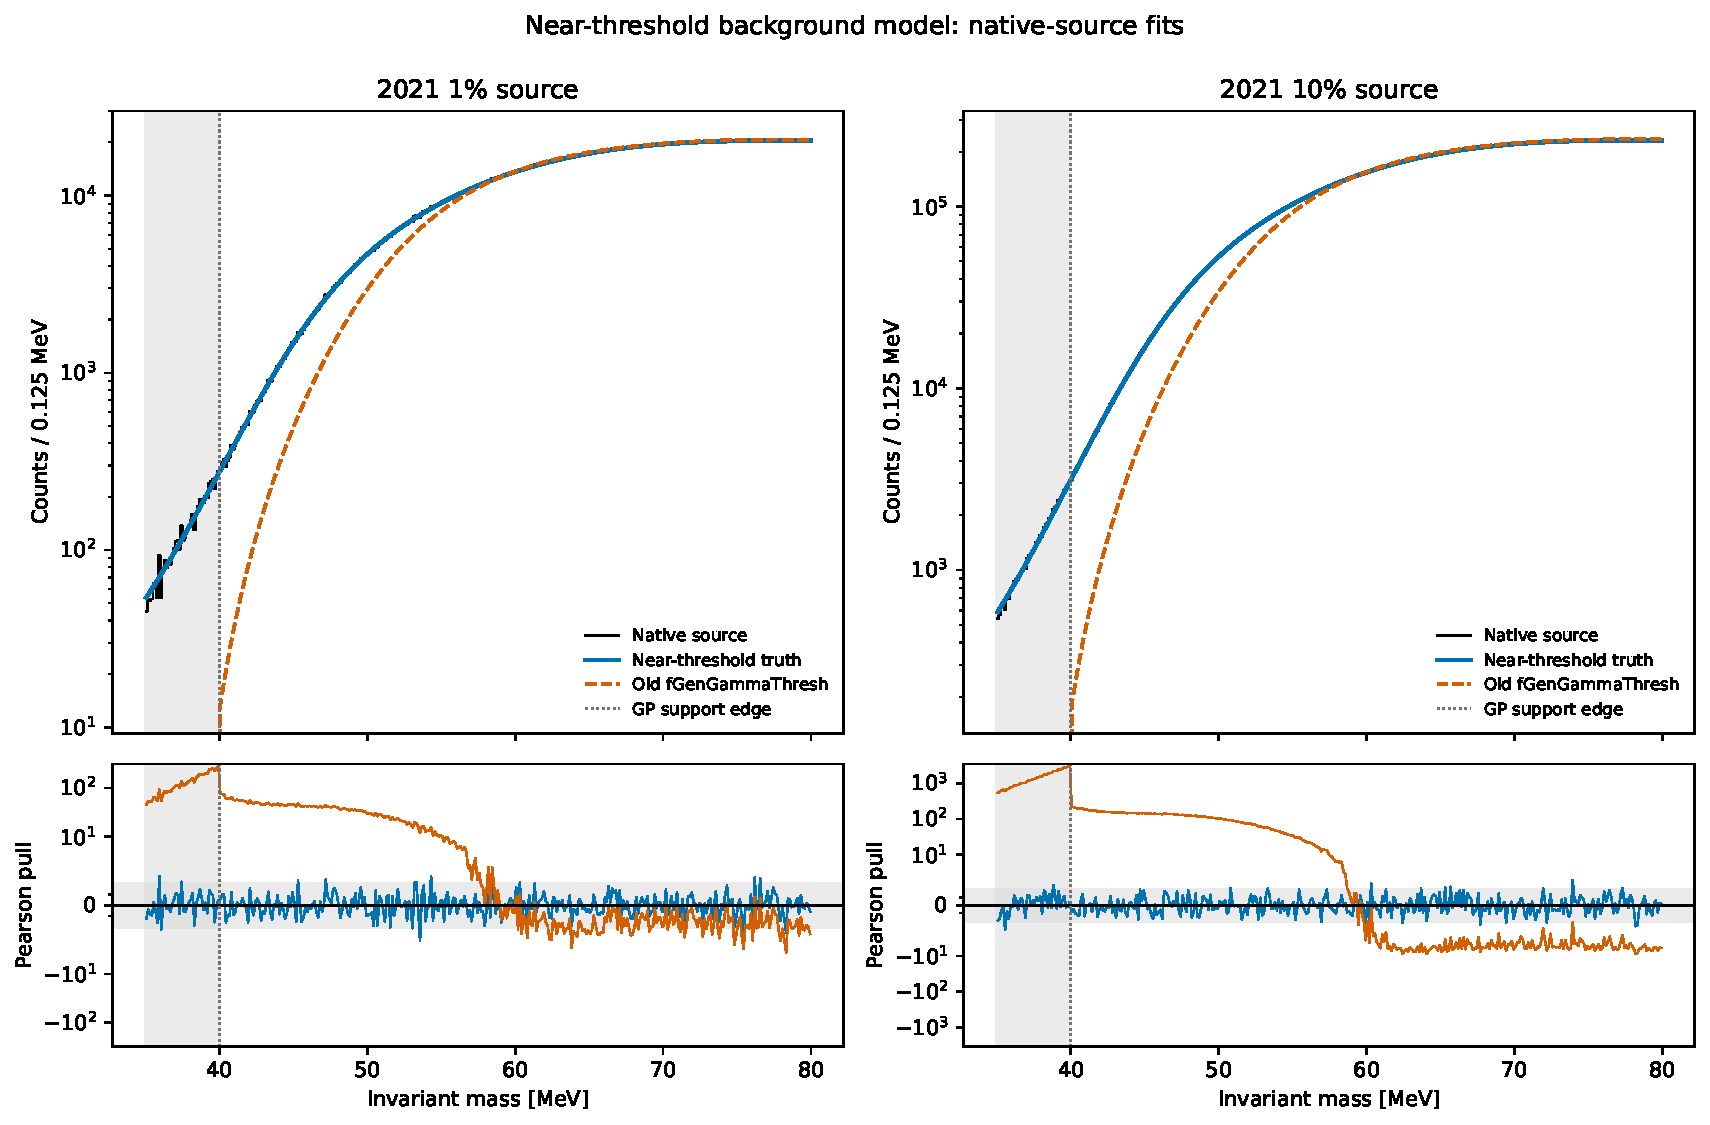
\includegraphics[width=0.98\linewidth]{../figures/history_writer/threshold_source_fits.pdf}
\caption{Historical source fits for the dedicated 2021 turn-on study.
Native 0.125-MeV source bins are compared with the local degree-five
model and the old generalized-gamma expectation. The local fit is shown
through 35--80~MeV, but the generated truth begins at 40~MeV and blends
to a rescaled tail from 75 to 80~MeV. The lower panels retain the large
old-model residuals on a symmetric-log scale. These are source-model
comparisons, not signal significances.}
\label{fig:v501-threshold-source}
\end{figure}

The new 20-background study reduced the $1\%\times10$ 65~MeV mean pull
to 0.300, with 95\% interval $[-0.219,0.819]$. Native 10\% retained
0.641, with interval $[0.082,1.199]$. Both scenarios had negative
55~MeV offsets, and $1\%\times10$ had a positive 70~MeV offset.
The old and new ensembles are unpaired and use different truths;
these results show partial conditional mitigation, not a universal
correction or a completed support choice.

\begin{figure}[p]\centering
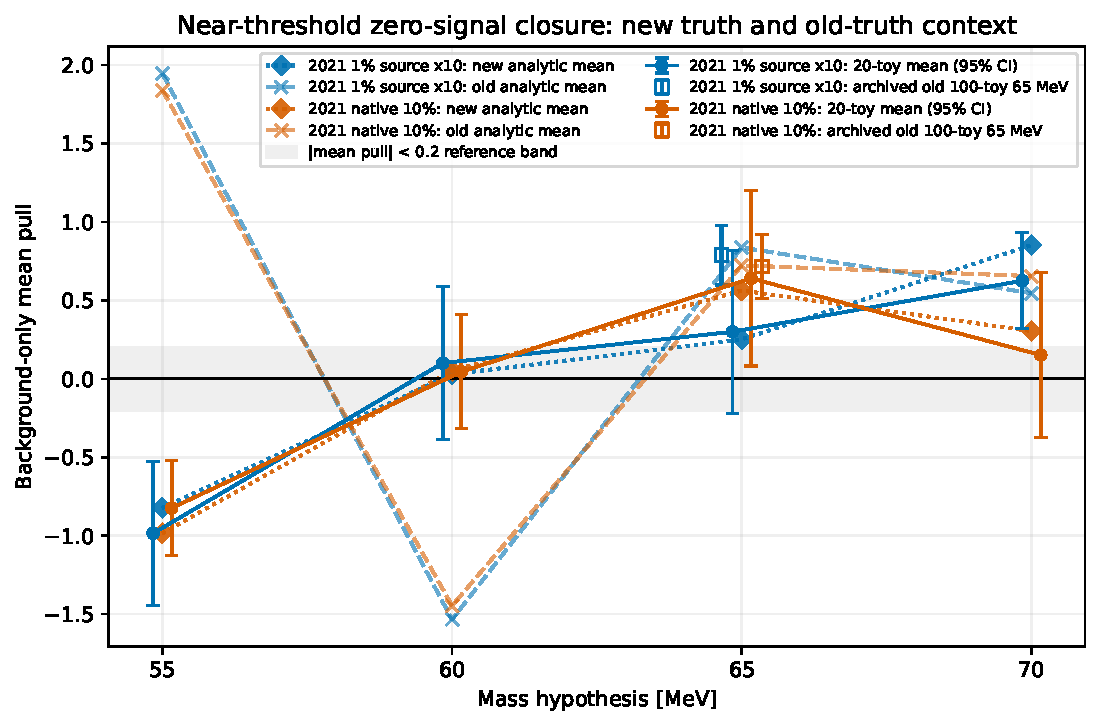
\includegraphics[width=0.98\linewidth]{../figures/history_writer/threshold_zero_signal.pdf}
\caption{Historical 20-background near-threshold closure. Points carry
95\% Student-$t$ intervals; deterministic responses to the old and new
analytic means expose the truth-shape dependence. The known 65~MeV
response improves in the 1\%-source test, while neighboring offsets
remain. The later 100-background replacement results in the main text
use their own identified truth and support; they are not pooled into
these curves.}
\label{fig:v501-threshold-zero-signal}
\end{figure}

Two later 65~MeV replacements entered the principal validation display.
The $1\%\times10$ replacement continued the degree-five turn-on study
to 100 backgrounds on 40--300~MeV support and gave mean pull 0.139
with 90\% interval $[-0.050,0.329]$. The native-10\% replacement used
the explicit degree-six intensity
\begin{equation}
 H_{10\%,6}(m)=S(m;t,w)
 \exp\!\left[\sum_{k=0}^{6}a_k
 T_k\!\left(\frac{m-0.055}{0.025}\right)\right]
 \label{eq:v501-native10-threshold}
\end{equation}
over 30--80~MeV, joined over 75--85~MeV to an archived
\texttt{fSigPowExpQ} tail with the same $q(u)$ but
$u=(m-0.075)/0.010$. It analyzed the full 30--300~MeV support. It gave $-0.246$ with 90\%
interval $[-0.417,-0.076]$; an independent continuation gave $-0.284$.
Its 85--300~MeV tail deviance/ndf remained 6.220. These replacements
explain the changed markers in the main plots, while preserving the
historical full-100 failure here. The later 36~MeV support decision is
a further, separately documented study.

\subsection{Controlled 2016 upper length-scale range}
\label{sec:v501-2016-upper-range}
The observed full-2016 study scanned upper factors
$k_{\max}=8,10,12,15,20$ at the same 142 hypotheses from 39 to 180~MeV.
A fit occupied the upper boundary when
$\ell_{\rm opt}/\ell_{\max}\geq0.999$. The occupancies were 142/142 at
factor eight, 56/142 at ten, and zero at twelve, fifteen and twenty.
This tested whether the imposed optimizer range was restricting the fit.

\begin{figure}[p]\centering
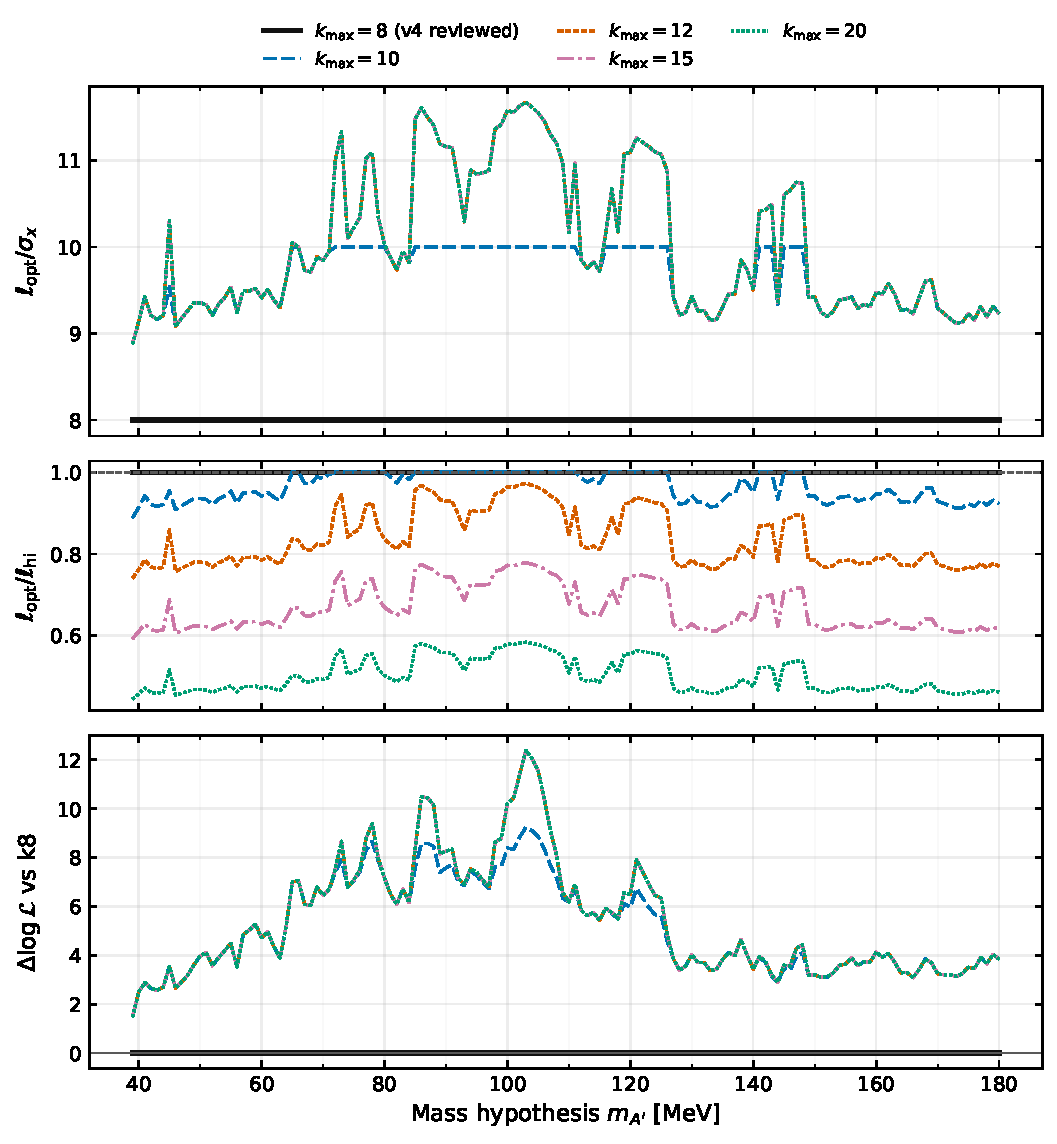
\includegraphics[width=0.96\linewidth]{../figures/history_writer/2016_upper_length_range.pdf}
\caption{The controlled 2016 upper-length-scale study, restored from
v4.9.7 Figure 74. The optimized scales, boundary occupancy and GP log
marginal likelihood are compared on identical data and mass hypotheses.
Factor twelve is the first nonbinding tested setting and is followed
by the factor-fifteen/factor-twenty plateau. This observed-data numerical
range diagnosis is not an expected-sensitivity or coverage optimization.}
\label{fig:v501-2016-upper-range}
\end{figure}

Questionable branches were repeated with the data and analysis card fixed.
Fourteen selected repair rows used the largest repeatable GP log marginal
likelihood; no limit, significance or kernel coordinate was interpolated.
From factor twelve to fifteen the largest observed-yield-limit change
was 0.083\%, the largest local-significance change was 0.00255, and
the log-marginal-likelihood differences lay in
$[-4.5,8.0]\times10^{-6}$. The fifteen-to-twenty comparison was similarly
stable. This supported factor twelve as the first nonbinding plateau
setting. The direction of the observed limit and the local p-values
were not selection criteria. Because the investigation followed an
observed boundary diagnosis, it is historical evidence for the range
choice, not a pre-unblinding freeze or a resolution of the later 2016
background-qualification exception.
